\subsection{Results}

The results gained from the TUBULAR flight can be broken down into the various subsystems as follows

\subsubsection{Mechanical Subsystem Performance}

\textbf{Structural Performance}

\smallskip
The frame structure and the aluminum walls withstood all the flight phases providing the required protection to all the components inside both boxes. 

Regarding the frame, the most critical load that it had to face was during landing. The gondola landed on the side where the boxes where allocated, thus they experienced a high load. Thanks to the use of bumpers as anchors of the boxes to the gondola rails and the styrofoam as a sitting surface, the force was damped, see Figures \ref{fig:bumpers_landing} and \ref{fig:styrofoam_landing}. Consequently the boxes did not move from its original place.

\begin{figure}[H]
    \centering
    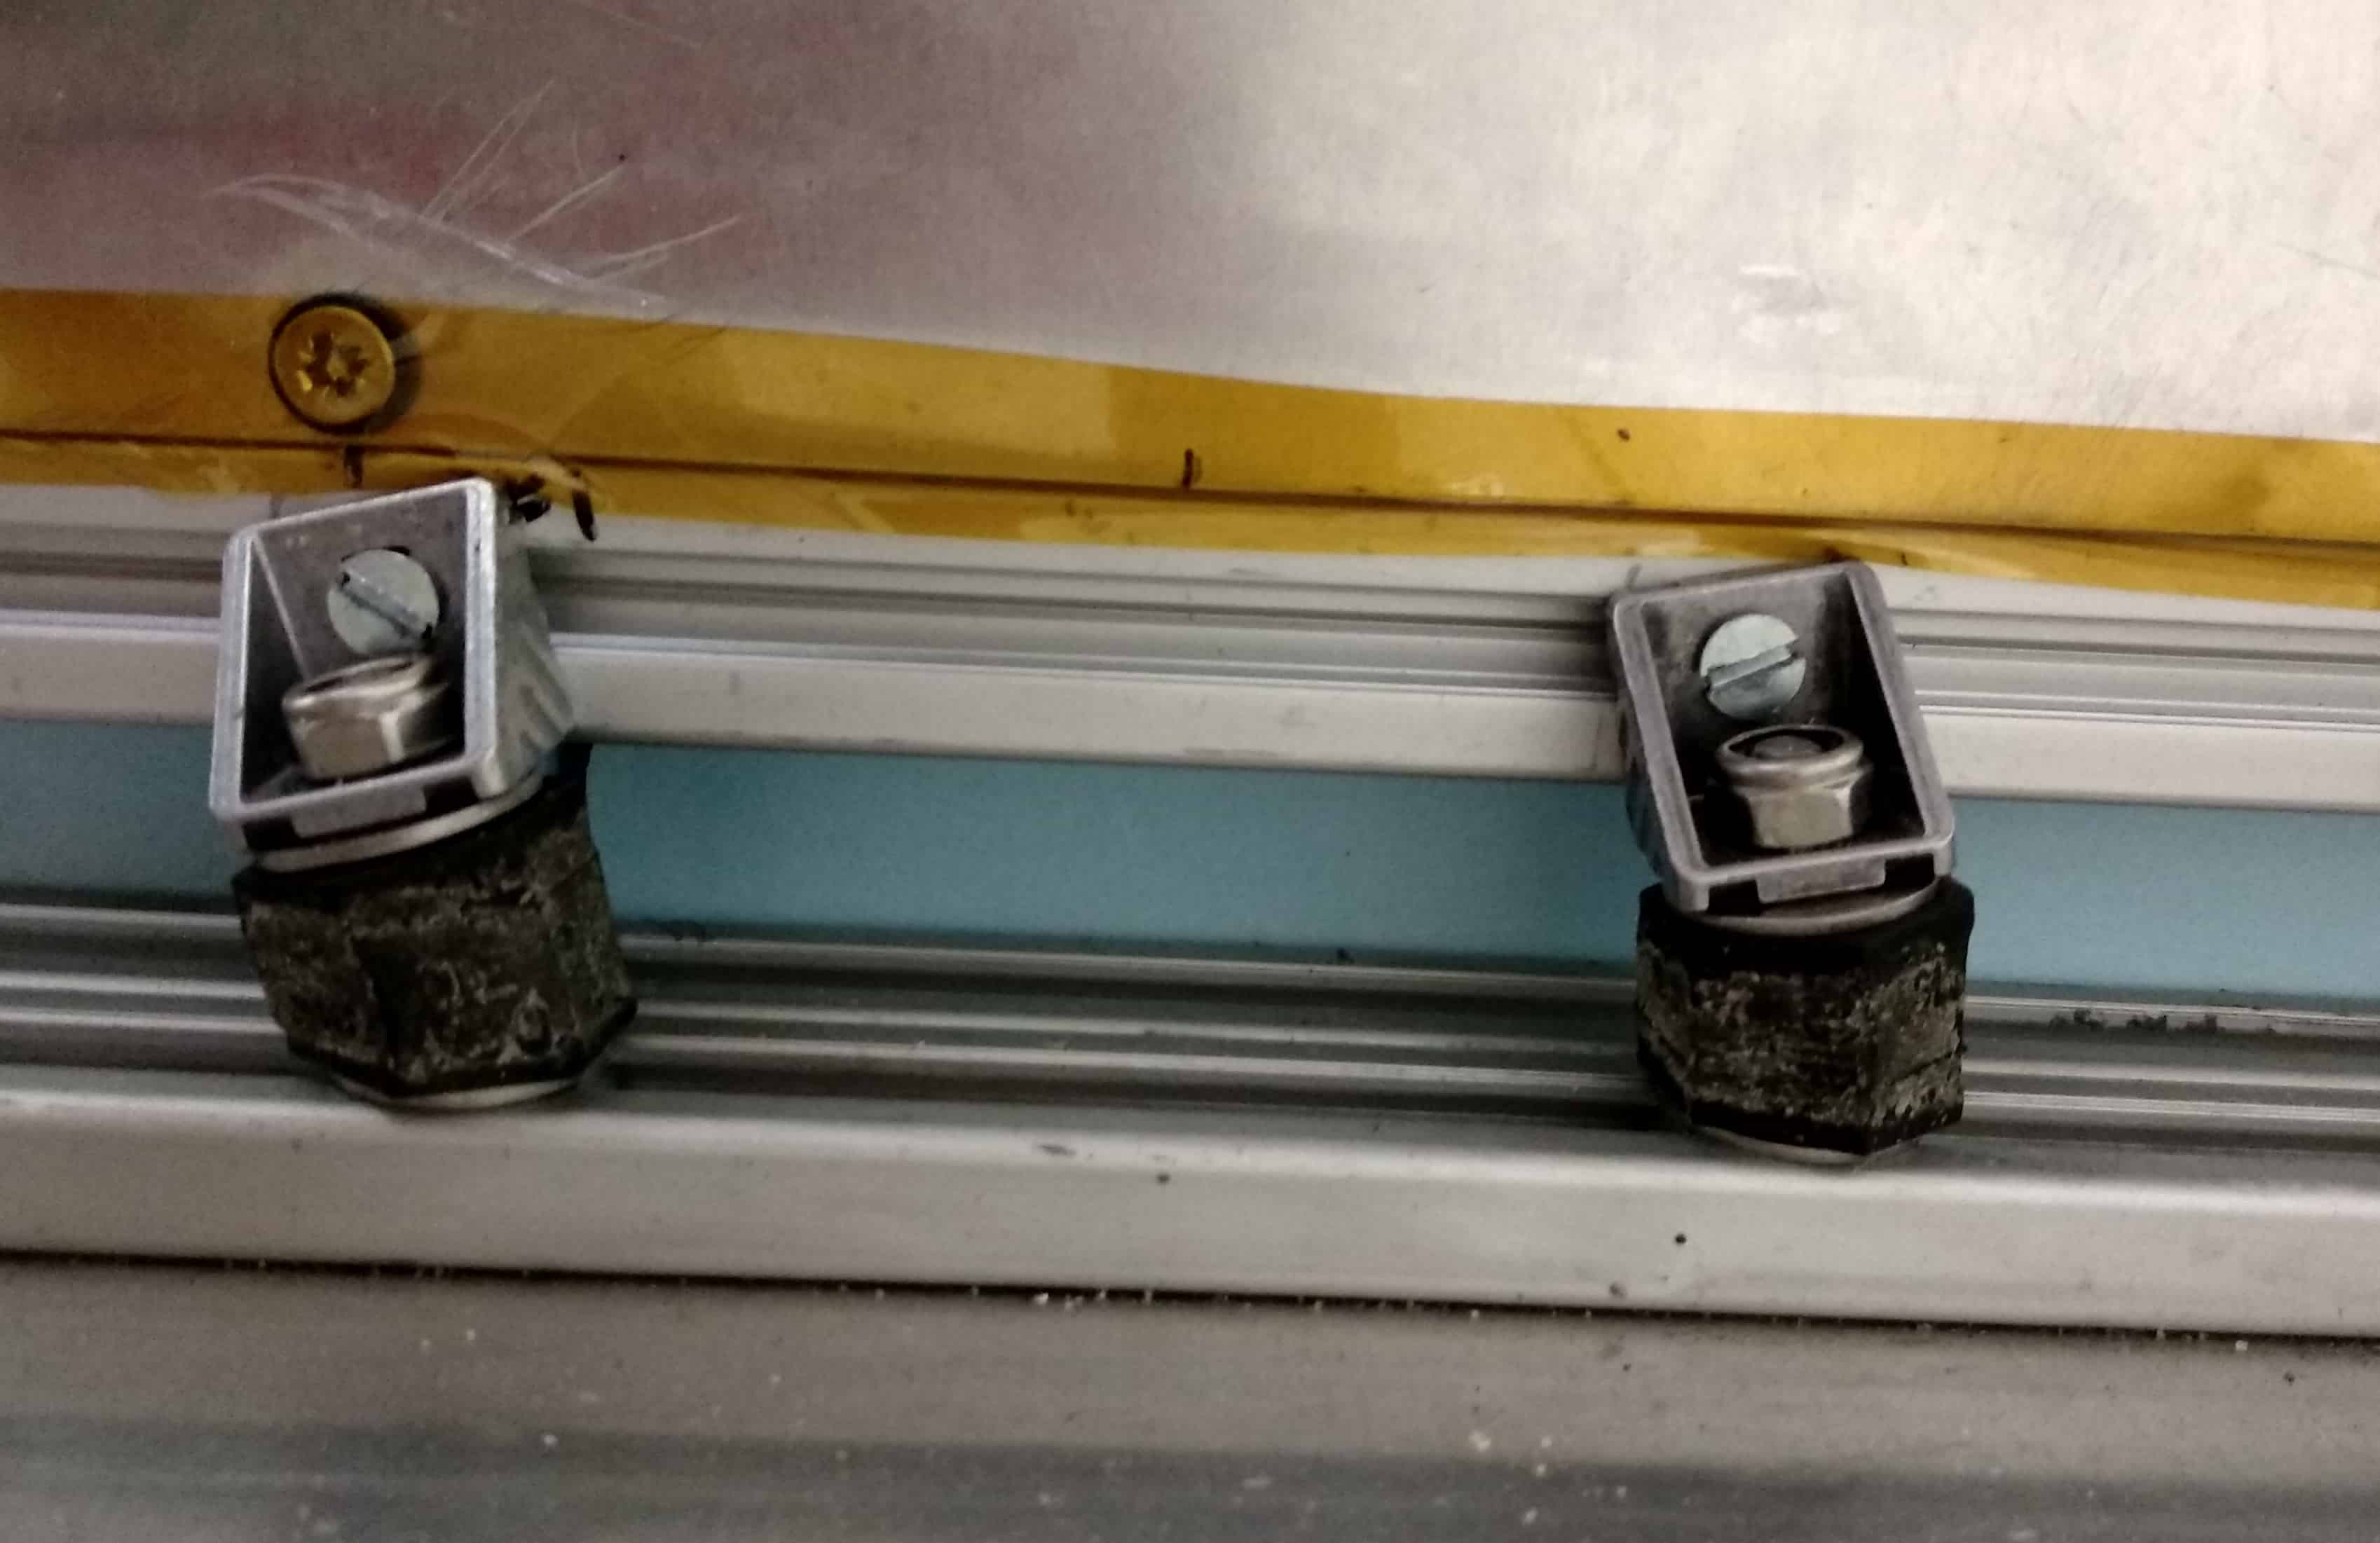
\includegraphics[width=0.8\textwidth]{7-data-analysis-and-results/img/Bumpers_Post_Flight.jpg}
    \caption{Position of the bumpers after landing.}
    \label{fig:bumpers_landing}
\end{figure}

\begin{figure}[H]
    \centering
    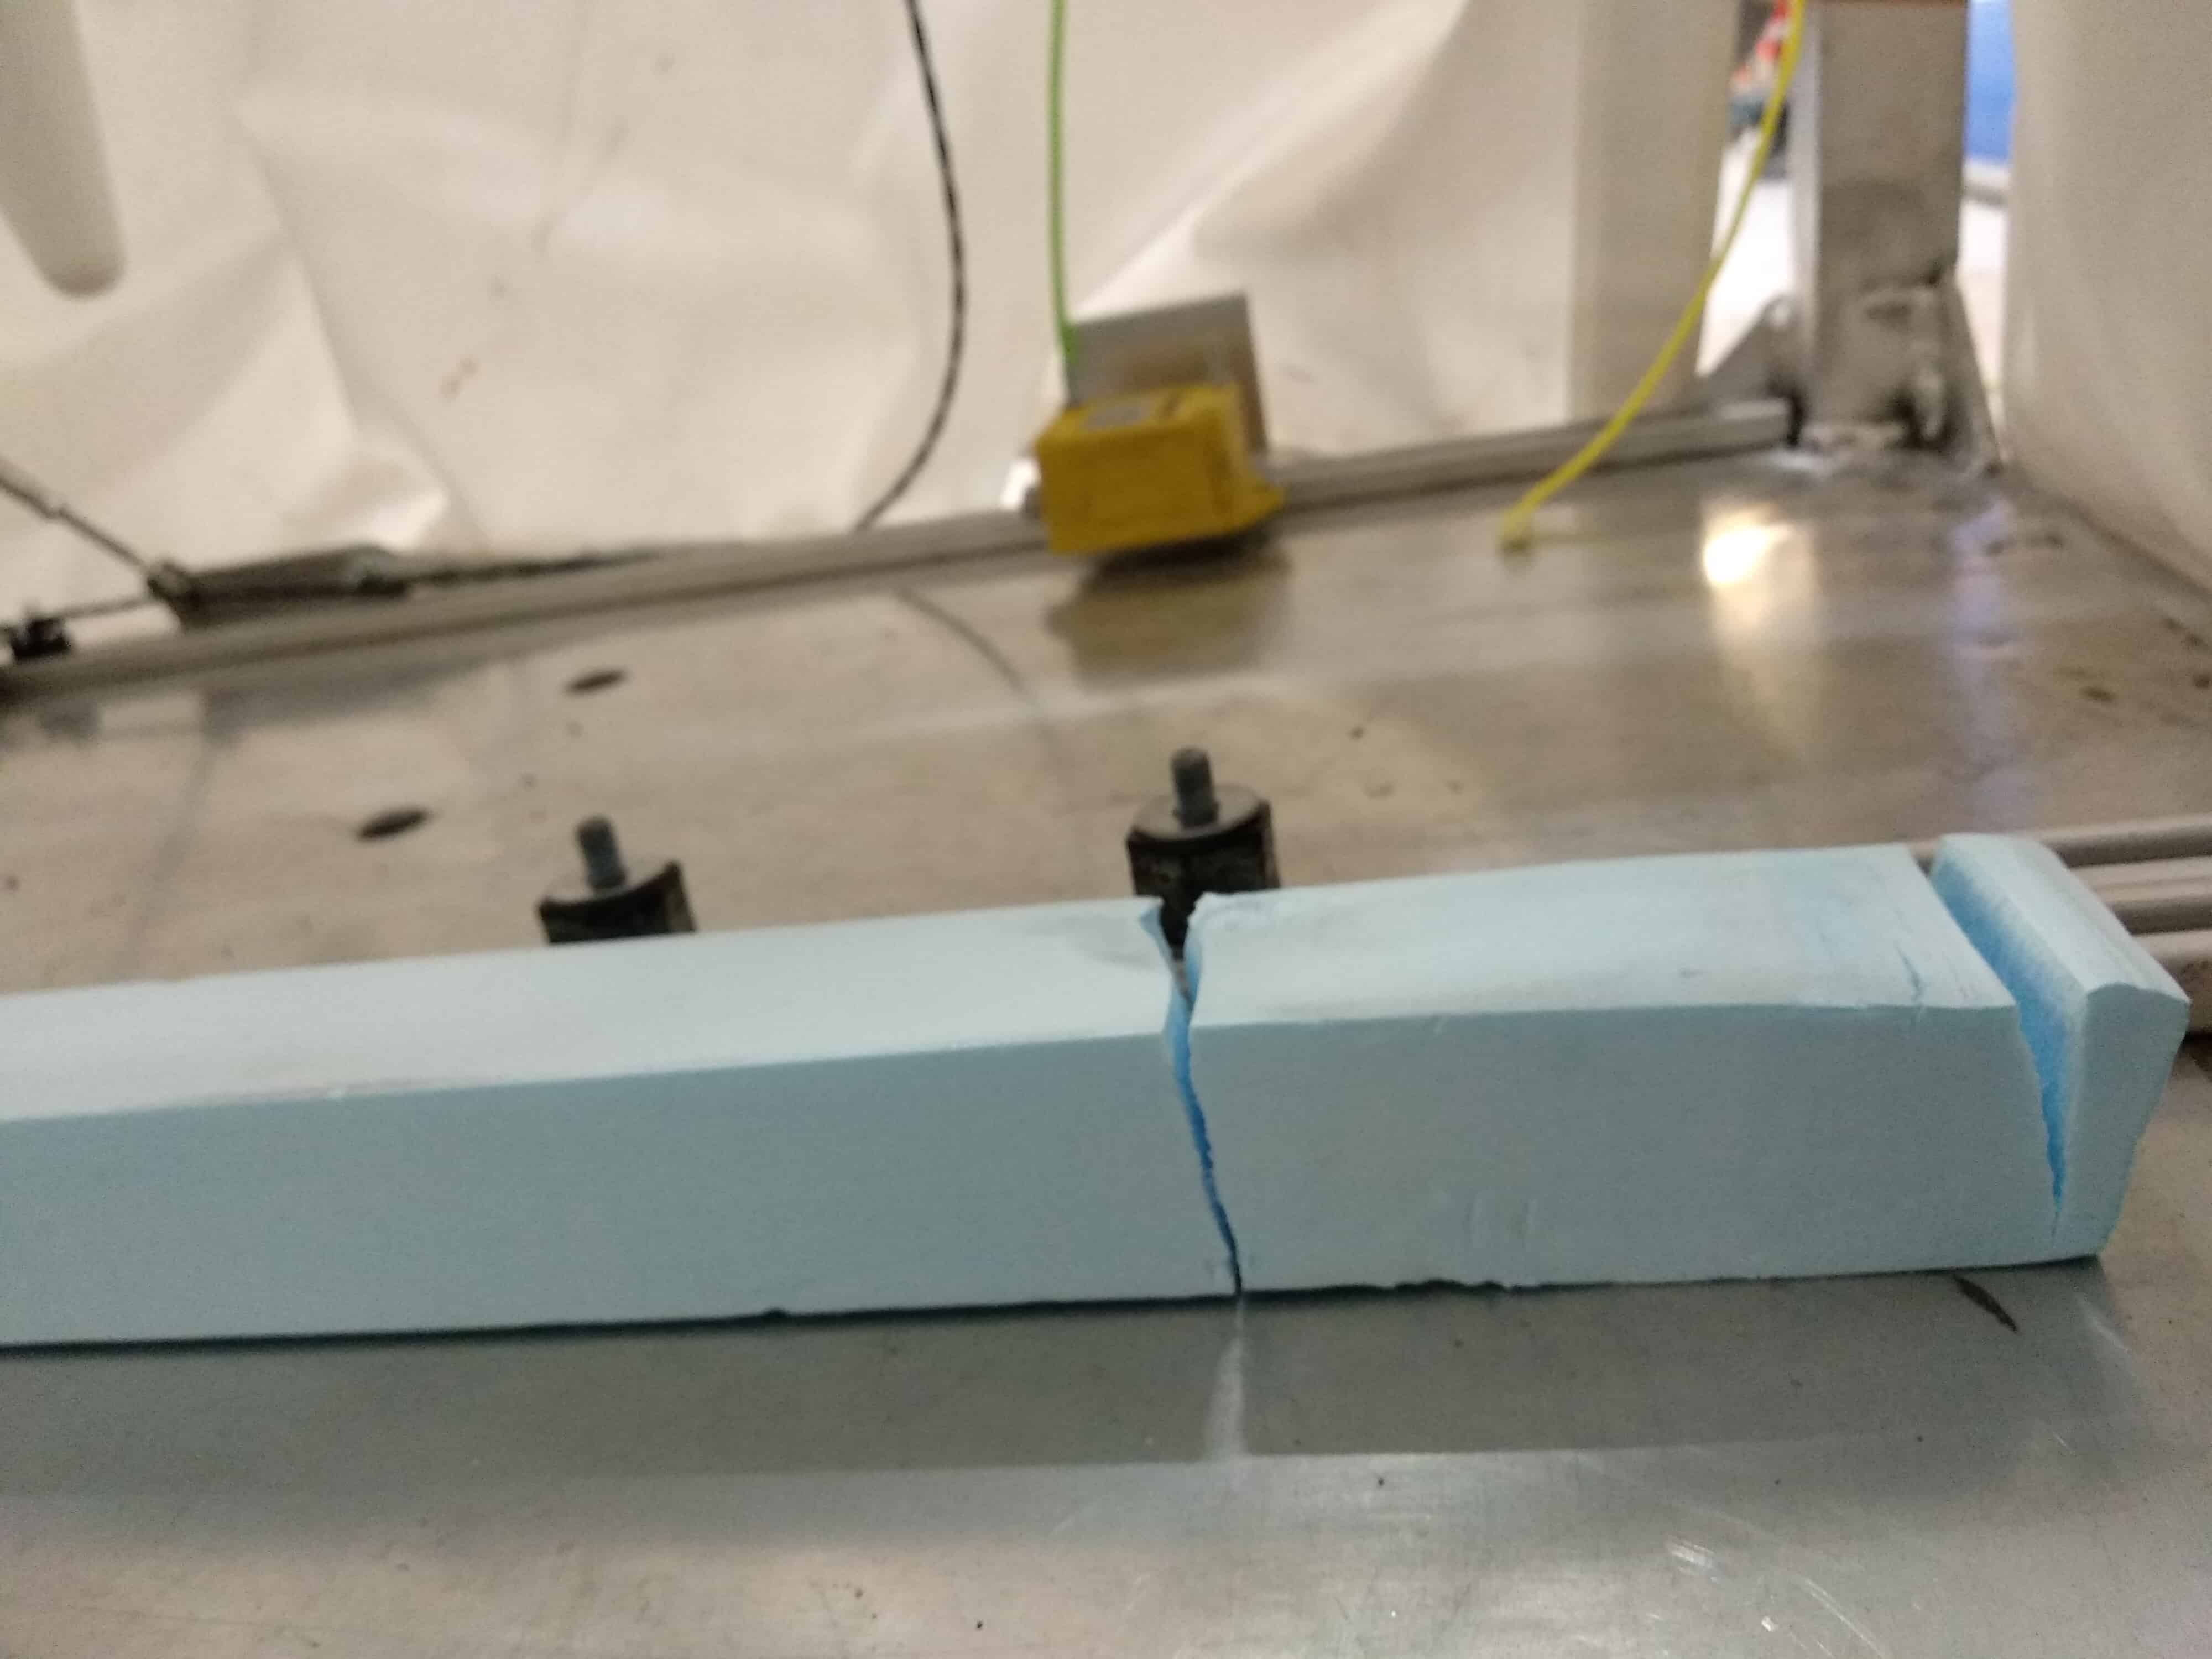
\includegraphics[width=0.8\textwidth]{7-data-analysis-and-results/img/Styrofoam_Post_Flight.jpg}
    \caption{Sytrofoam below the boxes after landing.}
    \label{fig:styrofoam_landing}
\end{figure}

The walls did not suffer any remarkable damage apart from the dirt that stuck to them as a cause of the sideways landing and some scratches from trees during landing. 


\textbf{Pneumatic circuit Performance}

\smallskip
The experiment had two separate pneumatic circuits, on each box. 

The air sampling with the CAC system was nominal. The valve opened and closed upon both automated and manual commands. This allowed to empty the 300-meter coiled tube during ascent and filling with stratospheric air during the descent phase.

On the other hand, the large pneumatic system of the AAC system experienced a failure in the pump which lead to the failure of the this alternative sampling system. Although the bags could not be filled with stratospheric air for later analysis, data of both airflow and pressure sensor was received as expected and all the valves worked nominally (manifold and flushing). 

The failure analysis of the pump can be found in Section \ref{post_flight}.

\subsubsection{Electrical Subsystem Performance}

Throughout the flight, none of the previous sensor dropouts that had been experienced were seen. This is thought to be due to the absence of larger electromagnetic interference's.

All other electrical parts worked as intended.

%However, during the campaign when all the teams were mounting their experiments onto the gondola and integration testing was underway, the digital communication lines started to react abnormally especially temperature sensors began to give unusual readings. After some investigation, the reason discovered behind this kind of behaviour was interference due to the close by wireless radio communication. The frequency at which the radio (walkie talkie) operating was actually charging up our experiment box. As a result, the grounding plane started to fluctuate between different levels which caused the experiment box to behave like an antenna. Because of this, once total communication black out between the experiment and ground station was witnessed. After getting familiar this with problem, the wireless radio communication has been avoided close to the experiment box. 
For details on the full failure analysis of the pump see Section \ref{sec:failureanalysis}.

\subsubsection{Software Subsystem Performance}
The software managed to control the experiment through the majority of the phases of the mission. The software worked even with frequent telemetry connection cutoff before the takeoff, during take-off it switched to Ascent mode successfully. When the failure with the pump occurred it successfully reset and put itself in the correct mode. Since sampling caused a reset it was decided that the software would be kept in Manual mode for the remainder of the flight.\par 
An unforeseen behavior was observed during descent when the choice was made to change the mode from Manual mode to Normal-Descent mode. Directly after this change a loss of communication happened before it reestablished itself a few seconds later, with all valves closed and the experiment in Standby mode. This is was indicative of a reset. Why it reset itself was most likely brought on by the fact the experiment passed several sampling points in Manual mode. Manual mode was thought to only be used for a short while and not to skip a sampling point. Incapable of taking a sample in Manual mode it is believed that the ASC performed a sampling when the software had the authority to do so, in which the pump was involved and therefor a reset happened. After the reset the software successfully went into Normal-Descent mode without taking a sample using the AAC. The choice was the made to take it into Safe mode which closed every valve successfully.\par
During the flight the only intermission of telemetry was during the reboot of the software after a reset. A permanent loss of telemetry happened at a low altitude due to limitations with line-of-sight. The on board software continued to record sensor data for several hours after landing. 

\subsubsection{Thermal Subsystem Performance}
\begin{figure}[H]
    \centering
    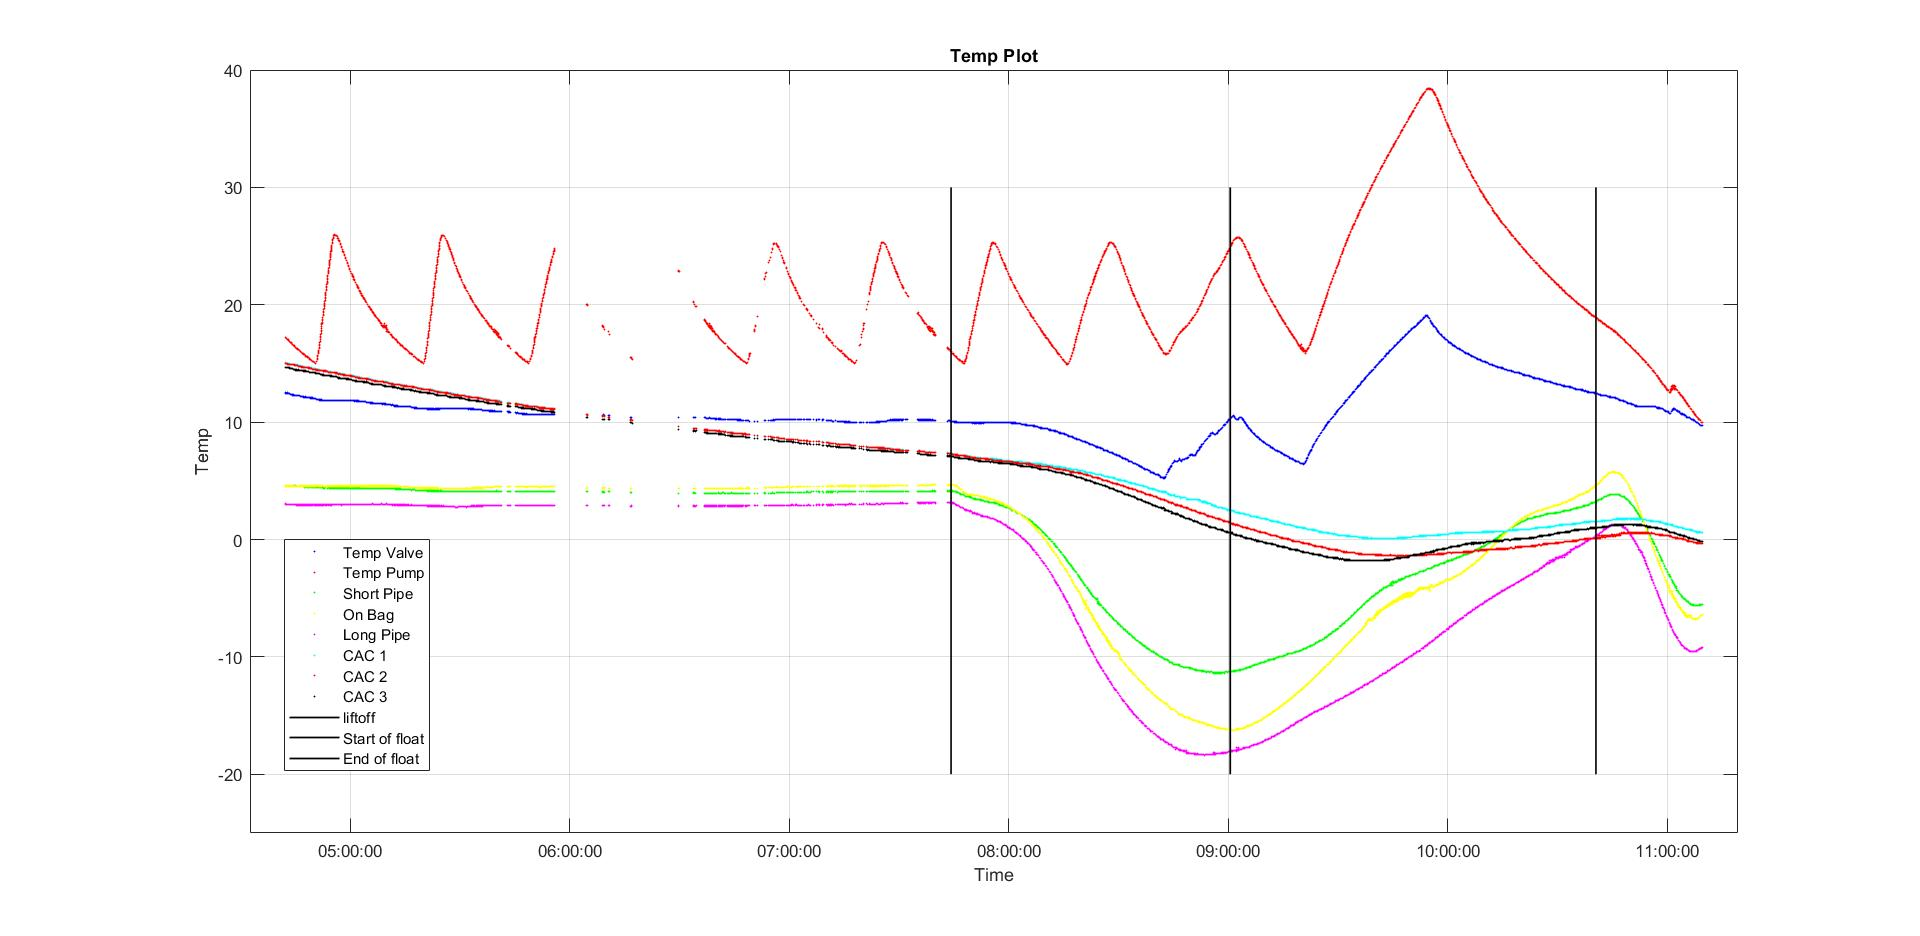
\includegraphics[width=\linewidth]{4-experiment-design/img/Termal_flight_true.jpg}
    \caption{The Temperature for the Different Sensors During Whole Fight.}
    \label{fig:Termal_flight_true}
\end{figure}
The thermal result for the flight are as seen in Figure \ref{fig:Termal_flight_true}. Both the critical components did not go lower than the operating threshold. The heaters operated as expected and kept the pump and manifold in their respective threshold limits. During the float phase a test were done to see if the pump issue were thermal related. The pump were then heated up to the upper limit and tried to start but did not work. It could then be concluded that the issue with pump during the flight were not thermal related. The simulations estimated the heaters would use 26.66Wh and during flight (calculated from Figure \ref{fig:Termal_flight_true}) 27.667Wh were used so the simulations were a good estimation.






\subsubsection{Scientific Results}\label{sec:scientificresults}
Raw data was only obtained on the 5th December therefore analysis is still ongoing and there are no official results as of yet. FMI has also sent over some preliminary results which can be seen in Figure \ref{fig:verticalprofiles}.

\begin{figure}[H]
    \begin{align*}
        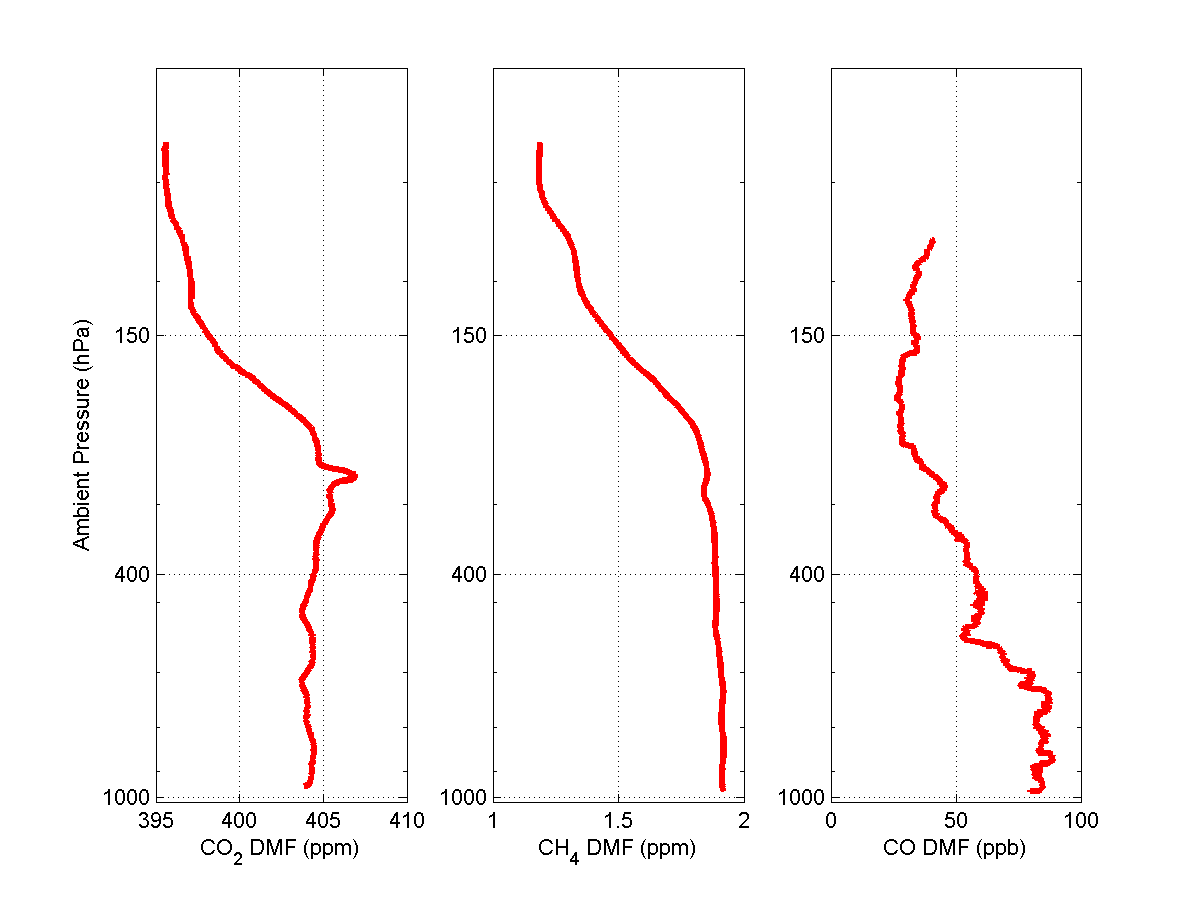
\includegraphics[width=1\linewidth]{7-data-analysis-and-results/img/verticalprofiles.png}
    \end{align*}
    \caption{Preliminary Vertical Profiles for (Left) CO$_2$, (Middle) CH$_4$, and (Right) CO.\label{fig:verticalprofiles}}
\end{figure}

As seen in Figure \ref{fig:verticalprofiles}, the preliminary results follow the general pattern of the expected results of the Section \ref{sec:ExpecterResults}. In general, the concentrations of CO$_2$, CH$_4$, and CO are decreasing with decreasing pressure i.e increasing altitude. The vertical axis represents the pressure but in the final profiles it will represent the corresponding altitudes. The maximum value of CO$_2$ is 405 ppm, for CH$_4$ is approximately 2 ppm, and for the CO is close to 90 ppb.  

The vertical resolution of the sample follow the one of the High-Resolution AirCore-HR (red line) in Figure \ref{fig:resolution-lenght} since the same length tube was used. Since the analysis was performed after 13 hours, the vertical resolution decrease is closer to the one represented by the green line in Figure \ref{fig:resolution-time}.

Further investigations are ongoing and the results will be updated. 

\subsubsection{Expected Results}
\label{sec:ExpecterResults}
After the analysis of the samples, the expected results were the vertical profiles of CO, CO$_2$, and CH$_4$. The profiles presented a similar pattern to that of Figure \ref{fig:vertical-profile-karion}. The continuous profile (dashed line) belongs to the CAC while the discrete values (black dots) belongs to the AAC (\cite{Karion}). Both profiles are showing a decrease in concentration of CH$_2$ and CH$_4$ with increasing altitude.
\begin{figure}[H]
    \begin{align*}
        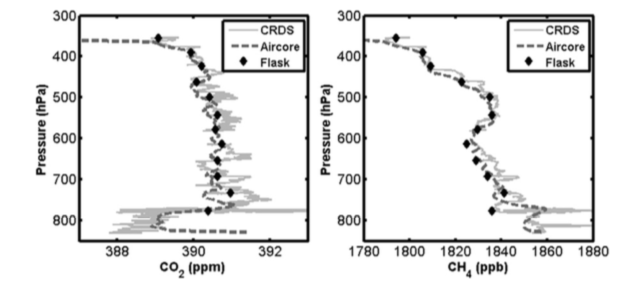
\includegraphics[width=1\linewidth]{7-data-analysis-and-results/img/ExpectedVerticalProfilesKarion.png}
    \end{align*}
    \caption{Pressure Profiles for (Left) CO$_2$ and (Right) CH$_4$ by Three Different Methods \cite{Karion}.\label{fig:vertical-profile-karion}}
\end{figure}

The experiment's goal was to achieve the highest vertical resolution possible. Since the vertical resolution was determined by the length and the diameter of the tube \cite{Membrive}, a 300 m long tube was used, consisting of 2 smaller tubes. One of 200 m length with \num{3e-3} m outside diameter and \num{1.3e-4} m wall thickness, and another one of 100 m length with \num{6e-3} m outside diameter and \num{1.3e-4} m wall thickness. For achieving higher stratospheric resolution, the tube with the smaller diameter was used to sample the higher altitudes and the one with the bigger diameter for the lower ones.
Figure \ref{fig:resolution-lenght} by Olivier Membrive \cite{Membrive} compares the vertical resolution that can be expected with three different AirCores.

\begin{figure}[H]
    \begin{align*}
        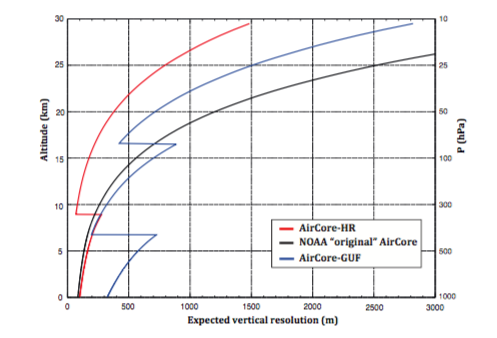
\includegraphics[width=1\linewidth]{7-data-analysis-and-results/img/ResolutionVslength.png}
    \end{align*}
    \caption{Comparison of the Vertical Resolutions That can be Expected with Different AirCores, After 3h Storage Time Before Analysis \cite{Membrive}.\label{fig:resolution-lenght}}
\end{figure}

The High-Resolution AirCore-HR (red line),\cite{Membrive}, is a combination of two tubes. One of 200 m and one of 100 m.

The NOAA 'original' CAC, \cite{Karion}, (black line) is a 152 m long tube and the AirCore-GUF (designed and developed at Goethe University Frankfurt), (blue line) is a combination of three tubes, 100 m long in total.

The longer AirCore, AirCore-HR, achieved a higher resolution throughout the whole sampled air. 

In addition, the vertical resolution depends on the the mixing inside the tube. 

The experiment takes into account two types of mixing. Molecular diffusion and the shear flow diffusion, known as Taylor dispersion. The effect of molecular diffusion is described by the root-mean-square of the distance of molecular travel, 
\begin{equation}
    X_{rms} = \sqrt{2Dt}
\end{equation}
where, D is the molecular diffusivity of the molecule in the surrounding gas, and t is the time over which travel occurs, \cite{Karion}.
For the tubing dimension that will be used in this experiment, the flow of air through the CAC, will be laminar. In such a flow, a parabolic velocity profile exists inside the tube, causing longitudinal mixing (Taylor dispersion). 

Before the experiment is recovered, only molecular diffusion will affect the sample, but during analysis both molecular diffusion and Taylor dispersion will affect the sample. Combining both of them, an effective diffusion coefficient can be calculated as,
 \begin{equation}
     D{eff} = D + \frac{a^2\overline{V^2}}{48D}
 \end{equation}
where D is the molecular diffusivity, a is the tube's inner radius, and $\overline{V}$ is the average velocity \cite{Membrive}. The first term translates into the longitudinal direction, while the second one is the Taylor dispersion. 

After completing Test 4 and Test 18 as seen in Tables \ref{tab:vacuum-test}, and \ref{tab:pump-low-pressure-test} respectively, the team managed to get the standard flow rate readings for the different altitudes. Standard flow rate is the volumetric flow rate of a gas corrected to standarized conditions of temperature and pressure. In this case the logged flow rates correspond to sea level conditions. Table \ref{tab:flow-rates} shows the standard flow rates at the sampling altitudes.  

% Please add the following required packages to your document preamble:
% \usepackage{multirow}
\begin{table}[H]
\centering
\begin{tabular}{|l|c|c|c|}
\hline
 & \multicolumn{1}{l|}{\textbf{Sampling Altitudes}} & \multicolumn{1}{l|}{\textbf{Ambient Pressure}} & \multicolumn{1}{l|}{\textbf{Standard Flow rate}} \\ \hline
\multirow{2}{*}{\textbf{Ascent Phase}} & 18 km & 75.0 hPa & $\sim$0.38 L/min \\ \cline{2-4} 
 & 21 km & 46.8 hPa & $\sim$0.21 L/min \\ \hline
\multirow{4}{*}{\textbf{Descent Phase}} & 17.5 km & 81.2 hPa & $\sim$0.41 L/min \\ \cline{2-4} 
 & 16 km & 102.9 hPa & $\sim$0.55 L/min \\ \cline{2-4} 
 & 14 km & 141.0 hPa & $\sim$0.79 L/min \\ \cline{2-4} 
 & 12 km & 193.3 hPa & $\sim$1.22 L/min \\ \hline
\end{tabular}
\caption{Sampling Altitudes as well as the Corresponding Ambient Pressures According to the 1976 US Standard Atmosphere and the Standard Flow Rates at Each Altitude.}
\label{tab:flow-rates}
\end{table}

It is necessary to also calculate the actual flow rates at the different altitudes. The conversion was done using the equation \cite{flowrateswebsite}:
$ Volumetric flow = (Standard flow rate) \cdot \Big(\frac{T_{alt}}{T_{std}}\Big) \cdot \Big(\frac{P_{std}}{P_{alt}}\Big) $
where, \\
$P_{std}= 1013 hPa$ is the standard pressure. \\
$T_{std}=294.25K$ is the standard temperature.\\
$T_{alt}$ is the temperature at the different altitudes.\\
$P_{alt}$ is the pressure at the different altitudes.\\

Table \ref{tab:normal-flow-rates}, shows the actual flow rates at the sampling altitudes.


\begin{table}[H]
\centering
\begin{tabular}{|l|c|c|c|}
\hline
 & \multicolumn{1}{l|}{\textbf{Sampling Altitudes}} & \multicolumn{1}{l|}{\textbf{Ambient Pressure}} & \multicolumn{1}{l|}{\textbf{Actual Flow rate}} \\ \hline
\multirow{2}{*}{\textbf{Ascent Phase}} & 18 km & 75.0 hPa & $\sim$3.78 L/min \\ \cline{2-4} 
 & 21 km & 46.8 hPa & $\sim$3.36 L/min \\ \hline
\multirow{4}{*}{\textbf{Descent Phase}} & 17.5 km & 81.2 hPa & $\sim$3.77 L/min \\ \cline{2-4} 
 & 16 km & 102.9 hPa & $\sim$3.99 L/min \\ \cline{2-4} 
 & 14 km & 141.0 hPa & $\sim$4.18 L/min \\ \cline{2-4} 
 & 12 km & 193.3 hPa & $\sim$4.71 L/min \\ \hline
\end{tabular}
\caption{Sampling Altitudes as well as the Corresponding Ambient Pressures According to the 1976 US Standard Atmosphere and the Normal Flow Rates at Each Altitude.}
\label{tab:normal-flow-rates}
\end{table}

Finally, storage time, that is the time from the moment the tube is sealed until the end of the analysis, is a key factor that affects the experiment's results in terms of resolution.

Figure \ref{fig:resolution-time} shows the effect of time delay between landing and analysis, on the expected vertical resolution. 
\begin{figure}[H]
    \begin{align*}
        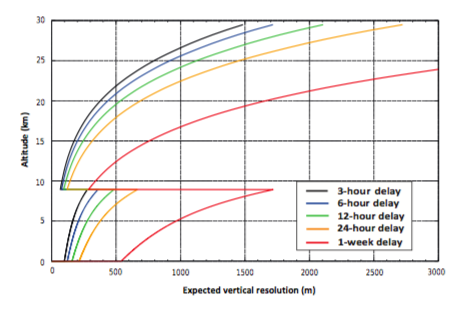
\includegraphics[width=1\linewidth]{7-data-analysis-and-results/img/ResolutionVsTime.png}
    \end{align*}
    \caption{Expected Vertical Resolution of AirCore-HR, for a Storage Time of 3h (Black), 6h (Blue), 12h (Green), 24h (Orange) and 1 Week (Red) \cite{Membrive}.\label{fig:resolution-time}}
\end{figure}

It is clear that the sooner the samples are going to be analyzed, the better the results for the vertical resolution of the CAC sample. At an altitude of 20 km the resolution decreases significantly from 300 m to 500 m for 6h and 12h of delay, respectively, \cite{Membrive}. But even after a week of storage, a vertical profile can still be achieved with lower resolution.

Based on past BEXUS projects, the time to experiment recovery is estimated at 12 to 24 hours, if not multiple days. As such, it is expected that the desired vertical resolution of gas analysis will favour AAC configuration over that of CAC due to mixing of gases in the latter configuration, resulting in poorer vertical resolution.

The vertical resolution for the AAC is approximately 500 m. This will be achieved assuring the airflow intake rate. For Ascent Phase, a nominal speed of 5 m/s is considered, which means that it will take 28.57 seconds to fill a sampling bag with 1.8L of air while ascending 142.85 m, and an  actual airflow intake rate of approximately 3.78 L/min at 18 km of altitude. For Descent Phase, the nominal speed is assumed to be 8 m/s. While descending 156.4 m a sampling bag will be filled in 19.55 seconds, with 1.3 L of air and an actual airflow intake rate of 3.99 L/min at 16 km of altitude. However, taking into account that the volume of the samples, at sea level, will be lower, the sampling time will be longer and the vertical resolution closer to 500m. 
%However, considering the fact that the pump will not have the same efficiency at higher altitudes, the sampling time may be longer and the airflow intake rate may be higher. The exact numbers will be included in the upcoming version of the SED.  

For a 500 m of vertical displacement, the horizontal resolution of the AAC has been approximated based on past BEXUS flights data obtained from the BEXUS manual \cite{BexusManual}. The average horizontal resolution obtained for Ascent Phase is 588m and for Descent Phase is 186.5 m. This means that the square area covered by the sample will be 500 m x 588 m and 500 m x 186.5 m for ascent and Descent Phases respectively.

It is expected that the AAC will serve as model enabling a cost-effective large scale deployment scheme for regular high altitude greenhouse gas measurement. Unlike CAC, the design of AAC will not impose experimental restrictions based on the proximity of infrastructure for shipping and analysis. As such, a successful proof of concept of AAC sampling system will serve as a basis to enable reliable cost-effective measurements in remote areas.


